\chapter{Planteamiento del problema}
%\pagenumbering{arabic} %Para empezar la numeración con números naturales

Actualmente para hacer la asignación de horarios, se reune el comité encargado de dicha tarea a realizar manualmente los esqueletos de los horarios. Éstos se dan a conocer a los profesores y ellos eligen diferentes opciones de materias y posibles horas en las cuales les gustaría impartir sus clases. Una vez que los profesores han hecho sus solicitudes, se vuelve a hacer una o varias juntas para la asignación final de los horarios que se hace de manera manual. Finalmente esta asignación de horarios se publica para los alumnos.

Con estos horarios, los alumnos llenan su tira de materias y van con cada profesor de la materia correspondiente para obtener la firma. El profesor firma si es que el cupo del salón lo permite. En caso de que el alumno no consiga la firma de la materia que desea, deberá buscar una segunda o tercera opción o incluso tener que meterla en algún semestre posterior. Es por ello que el trabajo que hemos realizado depende de la demanda de alumnos por materia y por horario.

%La principal razón por la cual los profesores no firman las tiras de materias es porque el número de alumnos que desean inscribirse a su clase es mayor al número de lugares disponibles en el salón asignado.

Por lo antes descrito, en este trabajo se pretende reducir el tiempo que toma la elaboración de los esqueletos de horarios y la asignación de grupos para las carreras del Departamento de Matemáticas. 

Esta aportación a la Facultad nos parece de gran utilidad y para beneficio de los alumnos. Además, el modelo propuesto puede ser aplicado para resolver problemas generales de asignación de recursos.

%Cabe aclarar que se tienen dos tipos de profesores, los de tiempo completo y los de asignatura. Los profesores de tiempo completo, por contrato, deben de cubrir ciertas horas de clase por lo que al momento de hacer la asignación se debe considerar que ellos requieren cubrir su solicitud.

En las siguientes secciones definimos los conceptos y nomenclatura que utilizaremos a lo largo del trabajo.

\section{Definición de conceptos}

%Las siguientes son las definiciones que se utilizarán a lo largo del trabajo:
  
\textbf{Materia:} Curso impartido en la Facultad por algún profesor.

\textbf{Horario:} Hora en la que se imparte alguna materia.

\textbf{Esqueleto:} Matriz con el número de grupos por hora y por materia.

\textbf{Asignación:} Matriz con las columnas Materia-Profesor-Horario.

\textbf{Grupo:} Vector con las entradas Materia-Profesor-Horario.

\textbf{Turno Matutino:} Comprende las clases impartidas de 7:00-14:00hrs incluyendo la clase de 14:00-15:00hrs.

\textbf{Turno Vespertino:} Comprende las clases impartidas de 15:00-21:00hrs incluyendo la clase de 21:00-22:00hrs.


\section{Nomenclatura}

$m:$ Número de materias, $m = 202$.
  
  $p:$ Número de profesores considerados, $p = 1223$.
  
  $t:$ Número de horas en las que se imparten las materias, $t = 15$.
  
  $i:$ Índice para profesores, $i \in \{ 1, 2, 3, \ldots, p \}$.
  
  $j:$ Índice para materias, $j \in \{ 1, 2, 3, \ldots, m \}$.
  
  $h:$ Índice para las horas del día, $h \in \{ 1, 2, 3 \ldots, t\}$.
  
  $U_{j,i,h}:$ Utilidad de que la materia $j$ sea impartida por  el profesor $i$ a la hora $h$.
  
  $x_{j,i,h}:$ Variable binaria que vale $1$ si la materia $j$ es impartida por el profesor $i$ a la hora $h$ y cero en otro caso.

$V_{j,i}:$ Variable binaria que vale $1$ si la materia $j$ puede ser impartida por  el profesor $i$ y cero en otro caso.

%$s:$ Semestre a simular

%$k:$ Número de semestres que se tienen como ventana de información.
%
%\textit{m\_grande:} Matriz en la que se guarda la información por semestres.

%$r:$ Matriz \textit{m\_filtrada}, submatriz de \textit{m\_grande}

%\textit{vec\_sem\_sig:} Vector con los semestres que se van a simular

%$num\_sim:$ Número de simulaciones de la demanda de alumnos para el semestre a simular.
  
%  $E:$ Matriz de $t$ renglones y $m$ columnas. En cada entrada se tiene la información del número de alumnos simulados en los grupos al crear \textit{mat\_esqueleto}.
%
%$D:$ Matriz de $t$ renglones y $m$ columnas. En la entrada $(i,j)$ se tiene la información de la demanda de alumnos para la hora $i$ y la materia $j$.
%
%$bin\_DUE:$ Matriz binaria de $t$ renglones y $m$ columnas. Tiene un 1 en la entrada $(i,j)$ si $E_{ij}$ o $D_{ij}$ tienen un valor distinto de cero. Tiene un cero cuando ambas matrices (D y E) tienen un cero en la entrada $(i,j)$.

%$:$ 
  %
%$:$ 
  %
%$:$ 
  %
%$:$ 
  %
%$:$ 
  %
%$:$ 
  
  
  \section{Planteamiento del problema de maximización}

En el problema de asignación de horarios se quiere asociar un profesor con una materia y un horario. Existen trabajos que han abordado este problema desde otro punto de vista, por ejemplo Yazdani, Naeri y Zeinali, en su artículo \textit{Algorithms for university course scheduling problems} [\ref{Yazdani}], proponen un modelo en el cual se toman 2 decisiones: la asignación de profesor por materia y el salón en el cual se va a impartir cada materia.

Con la función objetivo planteada en dicho modelo se desea maximizar la utilidad de que el profesor $i$ imparta la materia $j$, más la utilidad de que el profesor $i$ dé clases el día $d$, más la utilidad de que la materia $j$ sea impartida en el día $d$.

Nosotros abordaremos el problema considerando lo siguiente: %A continuación veremos las dos diferencias principales entre su modelo y el que proponemos en este trabajo.

\begin{enumerate}
\item[1)] Suponemos que todas las materias se imparten de lunes a viernes, a la misma hora, en el mismo salón. %No tomamos en cuenta el día en el que se imparte la materia.

\item[2)] Deseamos maximizar la utilidad de que la materia $j$ sea impartida por  el profesor $i$ a la hora $h$.
\end{enumerate}

%El problema que se tiene es un problema maximización en el cual se consideran:
El planteamiento del problema de maximización es el siguiente:

\begin{enumerate}[i)]
\item Variables de decisión:
  
  $ x_{j,i,h} =
  \begin{cases}
1  & \quad \text{si la materia } j \text{ es impartida por el profesor  } i \text{ a la hora } h\\
0  & \quad \text{e.o.c. } \\
\end{cases}
$
  
  \item Función objetivo (se desea maximizar la utilidad):

\begin{equation*}
\text{máx} \,\, z =  \,\, \displaystyle \sum_{i=1}^{p} \sum_{j=1}^{m} \sum_{h=1}^{t} x_{j,i,h} U_{j,i,h} \,\,\,\, \text{s. a}
\end{equation*}

\item Restricciones:
  
  \begin{eqnarray}
\displaystyle \sum_{i=1}^{p} \sum_{h=1}^{t} x_{j,i,h} &=& 1  \,\,\,\,\,\,\, \forall \,\, j\label{DarTodasMaterias}\\
\displaystyle \sum_{j=1}^{m} x_{j,i,h} &\leqslant& 1 \,\,\,\,\,\,\, \forall \,\, i,h \label{UnCursoXhora}\\
\displaystyle \sum_{h=1}^{t} x_{j,i,h} &\leqslant& V_{j,i} \,\,\,\,\,\,\, \forall \,\, j,i \label{ProfesorPuedeImpartir}\\
x_{j,i,h}, \,\, V_{j,i} &\in& \{0,1\} \,\,\,\,\,\,\, \forall \,\, j,i,h \label{VarBinarias}
\end{eqnarray}
\end{enumerate}

Con las restricciones del tipo (\ref{DarTodasMaterias}) aseguramos que todas las materias sean dadas. Con las del tipo (\ref{UnCursoXhora}) aseguramos que cada profesor no tenga más de un curso por hora. Con las del tipo (\ref{ProfesorPuedeImpartir}) aseguramos que los profesores tengan asignadas materias que puedan impartir. Finalmente con las restricciones del tipo (\ref{VarBinarias}) especificamos que las variables utilizadas son binarias.

%En el planteamiento se tienen dos tipos de restricciones: duras y suaves. Las restricciones duras son las que nos permiten tener soluciones factibles al cumplirlas en su totalidad y las restricciones suaves nos permiten evaluar la calidad de las diferentes soluciones. Usualmente las restricciones suaves están asociadas a preferencias y se cumplen en la medida de lo posible, pero no afectan la factibilidad de las soluciones.


Los elementos que consideramos en nuestro modelo son:
  
\begin{itemize}
\item[-] Esqueletos de horario: Matriz de $t$ renglones, correspondientes a las horas (7-8, 8-9, $\ldots$, 21-22) y $m$ columnas, una por cada materia. La entrada $(h,j)$ contiene el número de grupos simulados de la hora $h$ para la materia $j$.

\item[-] Función calificadora de esqueletos: Califica de acuerdo a qué tan bien o que tan mal se cubre la demanda de los alumnos esperados.

\item[-] Conjunto de materias: Nombres de las materias impartidas en la Facultad.

\item[-] Conjunto de profesores: Nombres de profesores de tiempo completo y de asignatura.

\item[-] Función calificadora de asignaciones: Califica con respecto al número de grupos simulados.
\end{itemize}

El conjunto de soluciones se presenta por medio de una matriz de tres columnas. El número de renglones depende del número de grupos que se hayan simulado. En el k-ésimo renglón se tiene la información de la k-ésima materia con su respectivo profesor y horario asignados. En la \tablename{~\ref{EjAsig}} se muestra un ejemplo del resultado de la asignación.

\begin{table}[H]
\centering
\resizebox{\textwidth}{!}{%
\begin{tabular}{|c|c|c|c|}
\hline 
\textbf{Materia} & \textbf{Profesor} & \textbf{Horario} \\ 
\hline 
Inferencia Estadística & Margarita Elvira Chávez Cano & 9 \\ 
\hline 
Modelos de Supervivencia y de Series de Tiempo  & Lizbeth Naranjo Albarrán & 13 \\ 
\hline 
Estadística Bayesiana  & Ruth Selene Fuentes García & 11 \\ 
\hline 
Modelos no Paramétricos y de Regresión & Jaime Vázquez Alamilla & 10 \\ 
\hline 
\end{tabular}}
\caption[\textit{Ejemplo de asignación}]{\textit{Se muestra un ejemplo de una asignación. La matriz tiene 3 columnas (Materia, Profesor, Horario).}}\label{EjAsig}
\end{table}




\section{Objetivos}

El primer objetivo del trabajo es hacer dos funciones que generen:
  
  \begin{enumerate}
\item[i)] Esqueletos de horarios

\item[ii)] Una asignación de profesores por materia y por hora.
\end{enumerate}


Los esqueletos de horarios son utilizados para simular una posible elección de materias y horarios de los profesores. La asignación debe cubrir la demanda de alumnos estimada para el semestre siguiente. Para generar los esqueletos de horarios se simula una posible solicitud de materias y horarios de los profesores.

El segundo objetivo es disminuir el tiempo utilizado actualmente para la realización de la asignación de horarios.


\section{Datos a analizar} \label{DatosAnalizar}

Para poder realizar el análisis de los datos, hicimos 4 grupos con respecto a dos criterios. El primer criterio fue con respecto al tipo de semestre, par o impar. El segundo criterio con respecto al turno, matutino o vespertino.

Para explicar la elección de los criterios tomamos la información de la materia \textit{Probabilidad I}, desde el semestre 2015-1 hasta el 2020-1. Dicha materia en la carrera de Actuaría es una materia obligatoria de tercer semestre. En las siguientes subsecciones veremos el análisis de acuerdo a cada criterio.

\subsection{Análisis por tipo de semestre: par e impar}

En la \figurename{~\ref{ParImparProbaI}} vemos que la línea azul representa el número de alumnos de los semestres impares y la línea roja representa el número de alumnos de los semestres pares. Observamos que en todo momento el número de alumnos de los semestres impares es mayor al número de alumnos de los semestres pares.

Ésto nos interesa porque al momento de simular debemos tomar en cuenta que el número de alumnos totales de semestres impares debe de ser siempre mayor al número total de alumnos de los semestres pares.

\begin{figure}[H]
\centering
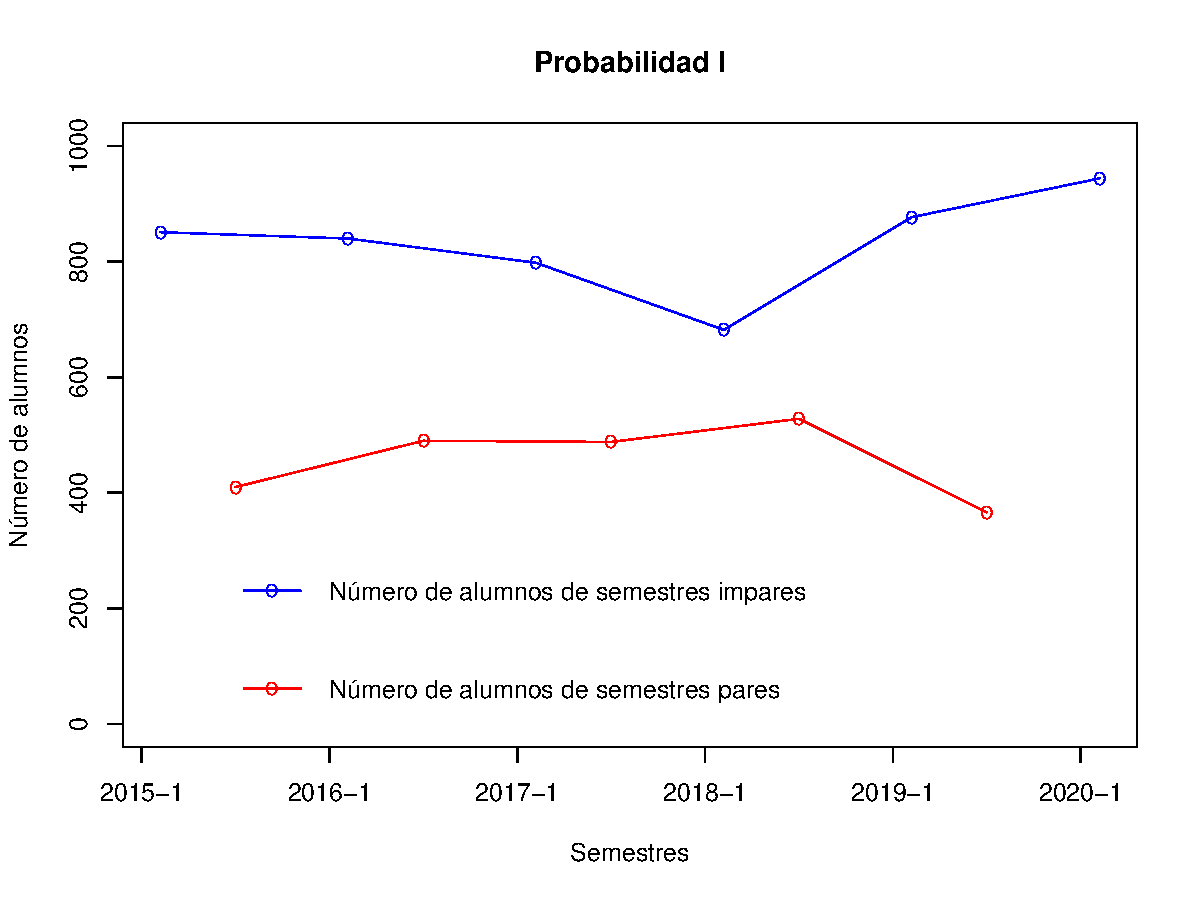
\includegraphics[scale = 0.7]{num_alum_sem_par_impar_Proba_I.pdf} %width=\textwidth
\caption[\textit{Número de alumnos por semestres pares e impares: Probabilidad I}]{\textit{Se muestran las series de tiempo del número de alumnos por semestres (pares e impares) de ``Probabilidad I''. Se puede observar que el número de alumnos de semestres impares es siempre mayor al de semestres pares.}}\label{ParImparProbaI}
\end{figure}

La \figurename{~\ref{HistAlumParImparProbaI}} contiene dos histogramas, las barras rojas representan el número de alumnos por grupo de semestres pares. Las barras azules representan el número de alumnos por grupo de semestres impares.

Las líneas que se encuentran sobre los histogramas son densidades estimadas que se ajustan a los datos. Para estas aproximaciones se ajustó un kernel gaussiano con la función \verb+density(X)+ de \textit{R}. Dicha función recibe como parámetro el vector $X$, con valores numéricos.

Algunos datos que se pueden obtener de las densidades vistas en la \figurename{~\ref{HistAlumParImparProbaI}} son por ejemplo que alrededor del $20\%$ de los grupos de los semestres pares tienen aproximadamente de $60$ a $70$ alumnos y que alrededor del $3\%$ de los grupos de los semestres impares tienen entre 150 y 180 alumnos. %\url{https://www.rdocumentation.org/packages/stats/versions/3.6.2/topics/density} %%Página con información de la función density de R

\begin{figure}[h]
\centering
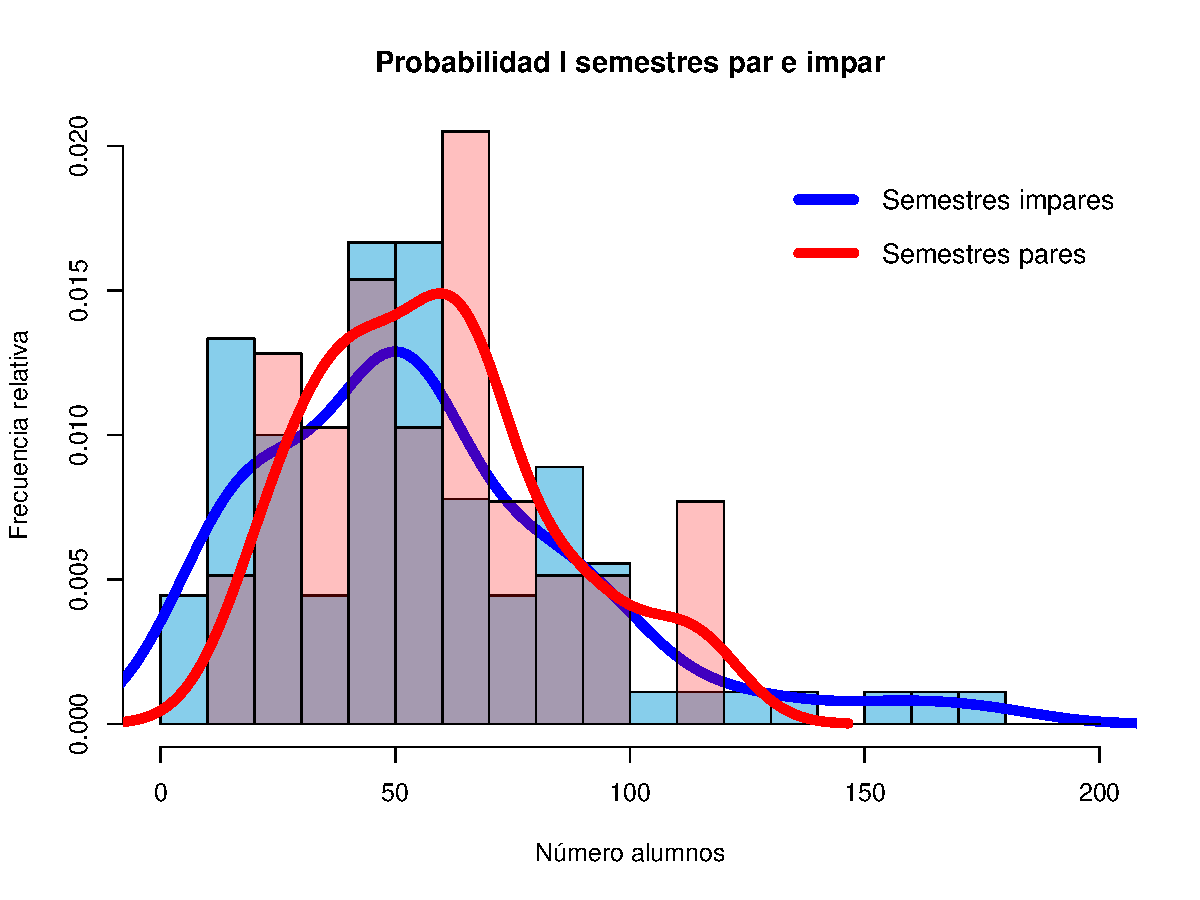
\includegraphics[scale = 0.7]{histograma_FR_num_alum_sem_par_impar_Proba_I.pdf} %width=\textwidth
\caption[\textit{Histogramas del número de alumnos por semestre: Probabilidad I}]{\textit{Se muestran los histogramas del número de alumnos por semestres (pares e impares) de ``Probabilidad I''. Se puede observar que las densidades ajustadas son muy parecidas.}}\label{HistAlumParImparProbaI}
\end{figure}

\subsection{Análisis por turno: matutino y vespertino}

En la \figurename{~\ref{num_alum_x_turno_Proba_I}} la línea azul representa el número de alumnos del turno matutino y la línea roja representa el número de alumnos del turno vespertino. Se puede observar que en todo momento el número de alumnos del turno matutino es mayor al número de alumnos del turno vespertino.

\begin{figure}[H]
\centering
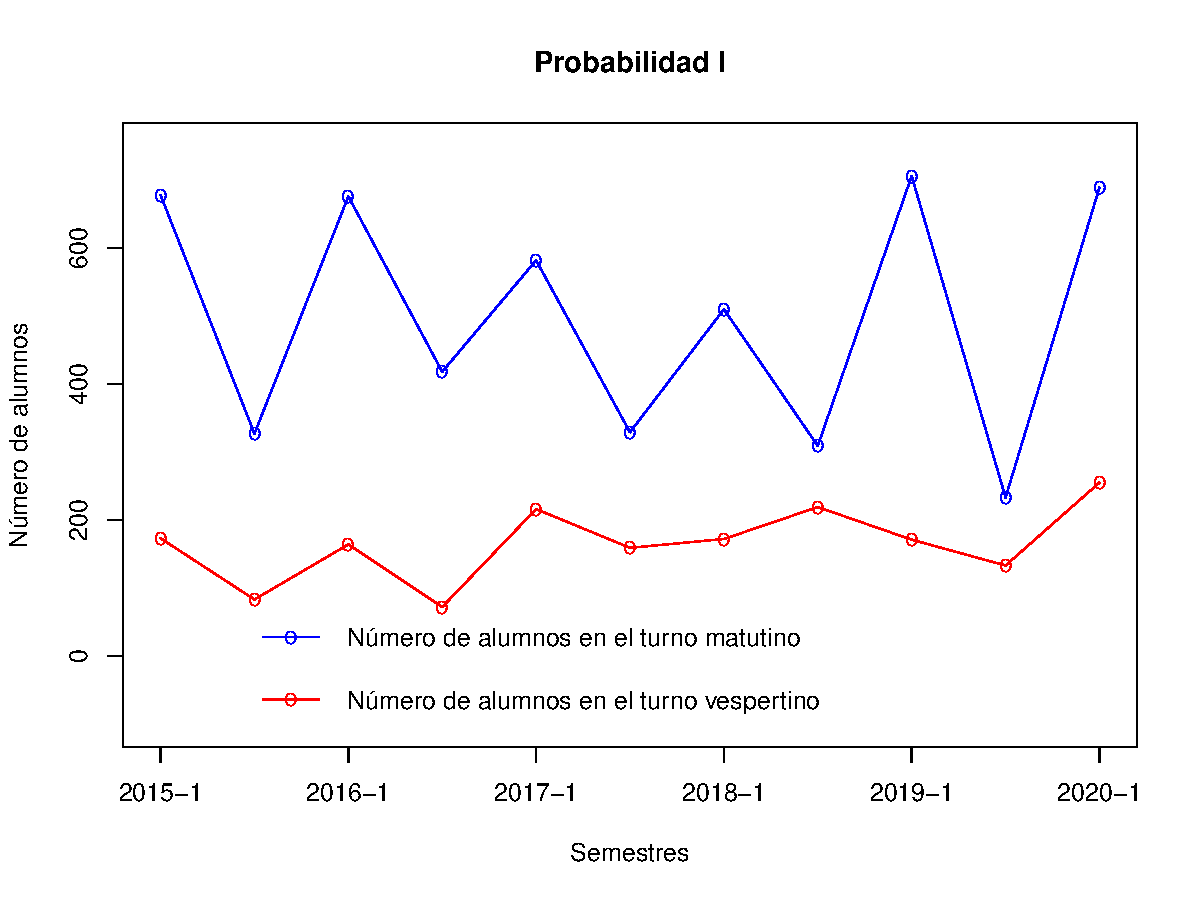
\includegraphics[scale = 0.7]{num_alum_x_turno_Proba_I.pdf} %width=\textwidth
\caption[\textit{Número de alumnos por turno: Probabilidad I}]{\textit{Se muestran las series de tiempo del número de alumnos por turno (matutino y vespertino) de ``Probabilidad I''. Se puede ver que el número de alumnos del turno matutino es siempre mayor al número de alumnos del turno vespertino.}}\label{num_alum_x_turno_Proba_I}
\end{figure}

También se puede ver que la varianza en el turno matutino es mucho mayor que en el turno vespertino. La desviación estándar del número de alumnos en el turno matutino es $179.20$ y en el turno vespertino es $54.95$. Ésto indica que en el turno vespertino se tiene prácticamente el mismo número de alumnos sin importar si la materia pertenece a un semestre par o impar. Por el contrario, en el turno matutino si influye el hecho de que la materia corresponda a un semestre par o impar.


%\begin{figure}[h]
%\centering
%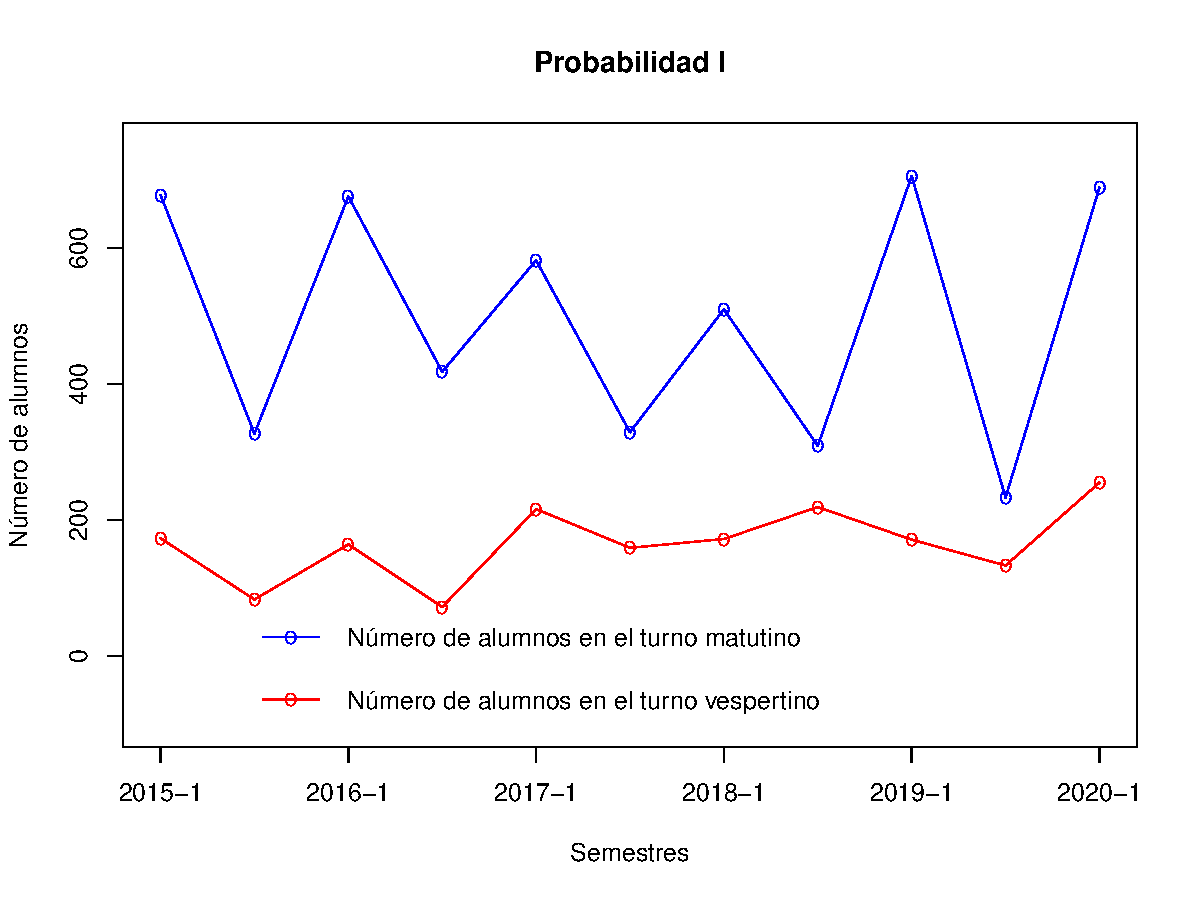
\includegraphics[scale = 0.7]{num_alum_x_turno_Proba_I.pdf} %width=\textwidth
%\caption[\textit{Número de alumnos por turno: Probabilidad I}]{\textit{Se muestran las series de tiempo del número de alumnos por turno (matutino y vespertino) de ``Probabilidad I''. Se puede ver que el número de alumnos del turno matutino es siempre mayor al número de alumnos del turno vespertino.}}\label{num_alum_x_turno_Proba_I}
%\end{figure}

En la \figurename{~\ref{HistAlumTurnoProbaI}} podemos ver dos histogramas, con las densidades ajustadas correspondientes. Las barras rojas representan el número de alumnos del turno vespertino y las barras azules representan el número de alumnos del turno matutino.

\begin{figure}[H]
\centering
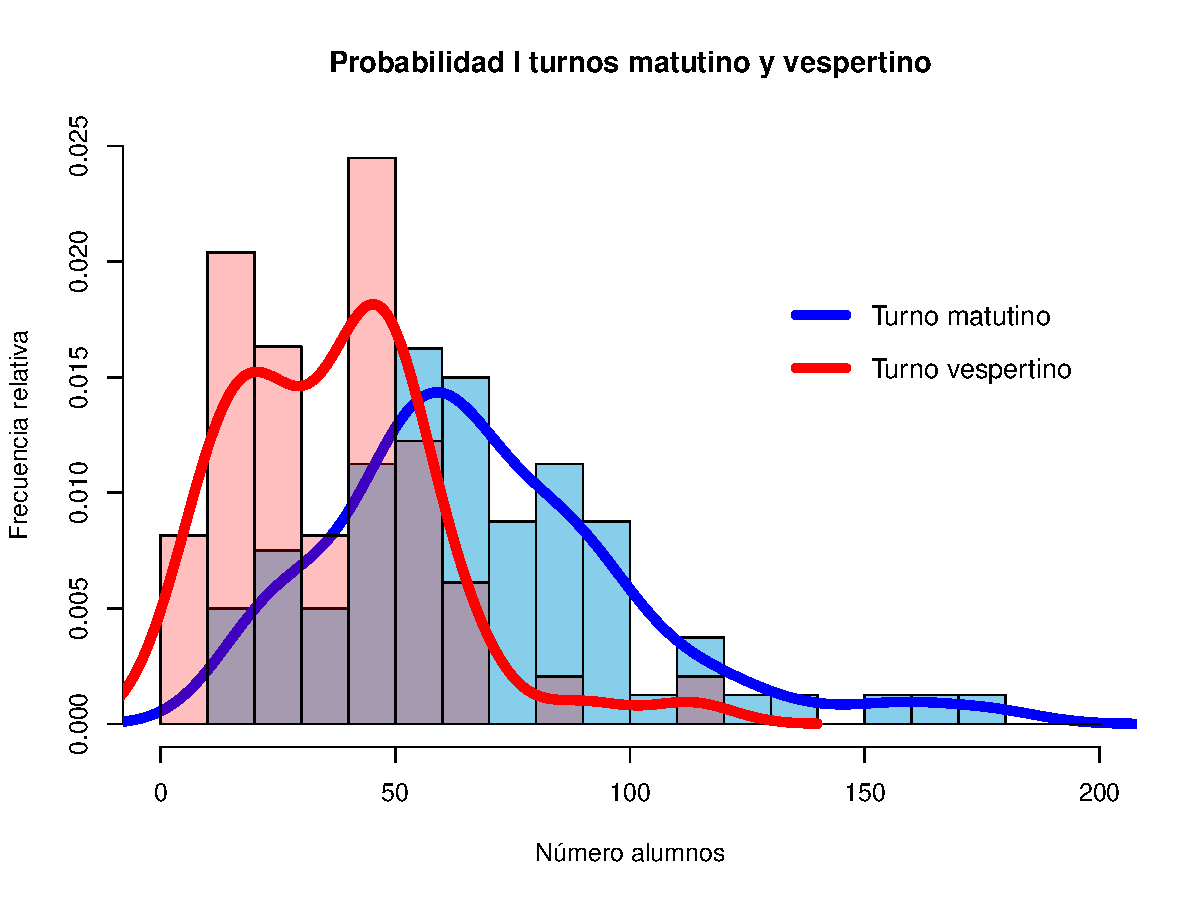
\includegraphics[scale = 0.7]{histograma_FR_num_alum_x_turno_Proba_I.pdf} %width=\textwidth
\caption[\textit{Histogramas del número de alumnos por turno: Probabilidad I}]{\textit{Se muestran los histogramas del número de alumnos por turno (matutino y vespertino) de ``Probabilidad I''. Se puede observar que las densidades ajustadas son muy diferentes.}}\label{HistAlumTurnoProbaI}
\end{figure}

En este caso las densidades ajustadas son completamente diferentes. Podemos ver que en el turno vespertino hay dos grandes concentraciones en los grupos que tienen entre 10 y 30 alumnos, así como entre 40 y 50 alumnos.

Algunos datos que se pueden obtener de las densidades ajustadas son por ejemplo que alrededor del $20\%$ de los grupos del turno vespertino tienen aproximadamente entre 10 y 20 alumnos y un poco más del $10\%$ de los grupos del turno matutino tienen entre 80 y 90 alumnos.

%\begin{figure}[h]
%\centering
%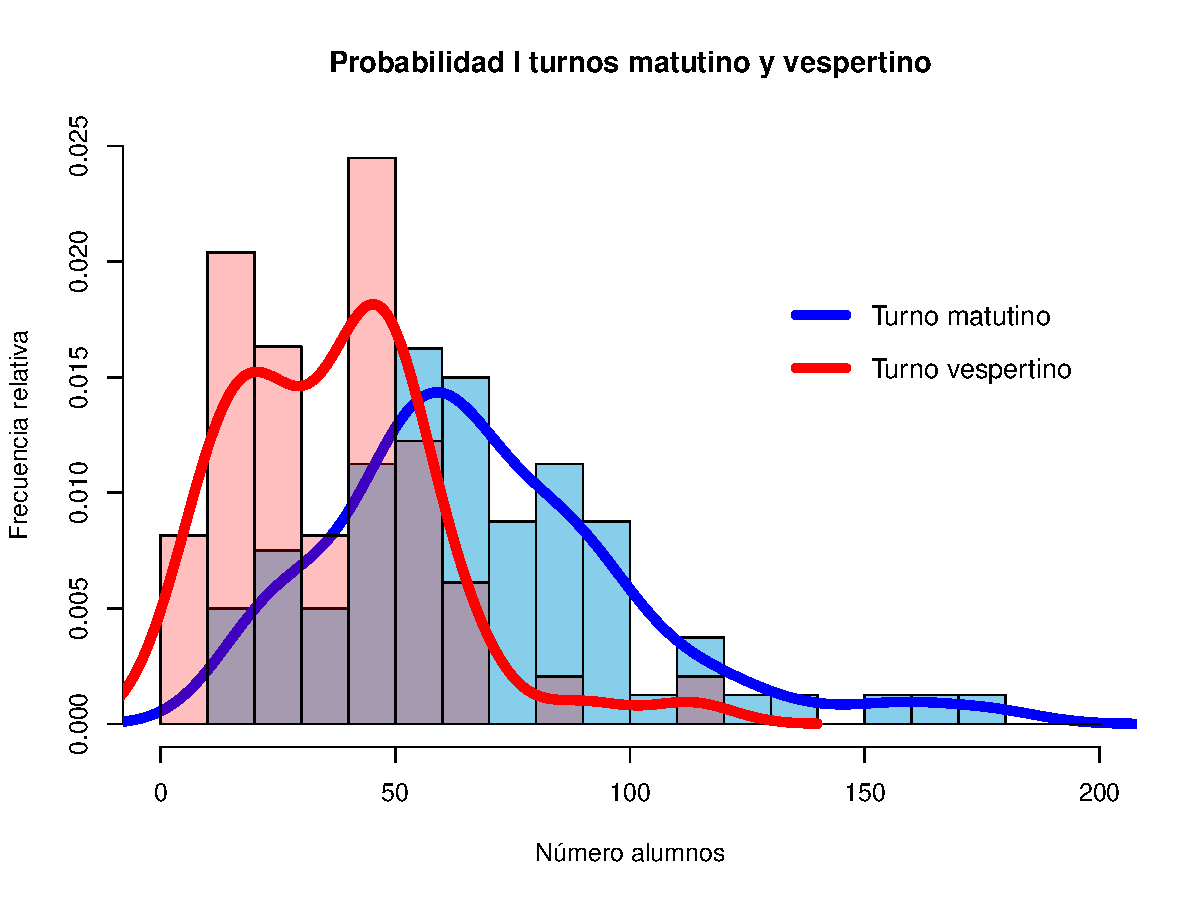
\includegraphics[scale = 0.7]{histograma_FR_num_alum_x_turno_Proba_I.pdf} %width=\textwidth
%\caption[\textit{Histogramas del número de alumnos por turno: Probabilidad I}]{\textit{Se muestran los histogramas del número de alumnos por turno (matutino y vespertino) de ``Probabilidad I''. Se puede observar que las densidades ajustadas son muy diferentes.}}\label{HistAlumTurnoProbaI}
%\end{figure}

Con los resultados obtenidos definimos los grupos de datos $G_{1}, G_{2}, G_{3}, G_{4}$, para hacer los análisis estadísticos, los cuales se muestran en la \tablename{~\ref{GposDatos}}.

\begin{table}[H]
\centering
\begin{tabular}{|c|c|c|}
\hline 
\textbf{Sem.} $\setminus$ \textbf{Turno} & \textbf{Matutino} & \textbf{Vespertino} \\ 
\hline 
Impar & $G_{1}$ & $G_{2}$ \\ 
\hline 
Par & $G_{3}$ & $G_{4}$ \\ 
\hline 
\end{tabular}
\caption[\textit{Grupos de datos}]{\textit{Se muestran los 4 grupos obtenidos al combinar los turnos (matutino y vespertino) con los tipos de semestres (pares e impares).}}\label{GposDatos}
\end{table}


